\documentclass[12pt, a4paper, final, fleqn]{article}
\usepackage{graphics, graphicx}
\usepackage{amsmath}
\usepackage{microtype}
\usepackage[english]{babel}
%\usepackage[round,numbers,comma,sort&compress]{natbib} % references as numbers
\usepackage[square,numbers,comma]{natbib} % refereces as text
\usepackage{a4wide}
\usepackage[normalem]{ulem}
\usepackage[colorlinks,citecolor=blue,filecolor=black,linkcolor=black,urlcolor=black]{hyperref}
\usepackage{color}
\usepackage{array}
\usepackage{colortbl}
\usepackage{tabularx}
\usepackage{booktabs}
\usepackage{lineno}
\usepackage{caption}  % to put caption outside figure env -- used for text boxes
\usepackage{setspace}  % to use double spacing
\usepackage{marginnote}  % to put margin notes with glossary
%\usepackage{framed}
\usepackage[top=1.5cm, bottom=1.5cm, outer=5cm, inner=2cm, heightrounded, marginparwidth=3.6cm, marginparsep=0.8cm]{geometry}
\graphicspath{{figures/}}
\newcommand{\comment}[1]{}
\definecolor{nero}{rgb}{0., 0., 0.}
\definecolor{bianco}{rgb}{1, 1, 1}
\definecolor{andrea}{rgb}{0., 1., 1.}
\definecolor{grigio}{rgb}{.4, .4, .4}

\newcommand{\discA}[1]{\textcolor{andrea}{\sout{#1}}}
\newcommand{\chngA}[1]{\textcolor{andrea}{\textsf{\textbf{#1}}}}

\newcommand{\dd}{\mathrm{d}}
\newcommand{\transp}{\dag}

% create a framed margin note with colored frame and first word bold face 
\newcommand{\glossarybox}[2]{\marginnote{\fcolorbox{cyan}{white}{\begin{minipage}{0.25\columnwidth}\scriptsize{\textbf{#1:} #2}\end{minipage}}}}

\begin{document}

\begin{center}

\vspace*{2cm}

%{ \Large {\bf The metacognitive filter}}
{ \Large {\bf The topology of mental states.} \\
Combining data science and graph theory to reveal neural networks for cognitive functions.}


\vspace*{2cm}

\large
Andrea Insabato\\[1 cm]

\normalsize
{Universitat Pompeu Fabra \\
Theoretical and Computational Neuroscience\\
Center for Brain and Cognition \\
Roc Boronat, 138\\
08018 Barcelona, Spain,} \\[1 cm]

\normalsize
{Columbia University \\
Italian Academy for Advanced Studies
Center for Theoretical Neuroscience\\
1161 Amsterdam Ave.\\
New York NY 10027, USA} \\[1 cm]

\end{center}

\vfill
Keywords:  machine-learning; classification; effective connectivity; functional connectivity; features selection; dimensionality reduction\\
\today


\newpage
%\linenumbers
\doublespacing
\begin{abstract}
This is the abstract.
\end{abstract}

\newpage
\tableofcontents
\newpage
\section{Introduction}
\label{intro}

This article is meant to be a general introduction to the study of cognitive functions and dysfunctions
from the perspective of data science and network science.
While the idea of the brain as the physical substrate of \emph{mental} activity is quite old and more or
less well established and the idea of the brain as a network of interconnected units is, although not as old,
probably more widespread and shared, the study of whole brain networks underlying cognitive functions and brain disorders
is only becoming possible very recently thanks to the acquisition of huge amount of data (often referred to as ``big data'')
and to the development of adequate quantitative methods to analyze such data.
\glossarybox{fMRI}{the activity of neurons is visualized through the
induced magnetic field. Current spatial resolution of fMRI is in the order of
mm, allowing to study large ensables of neurons such as hypercolumns.}
The specific focus adopted here will be on estimating connectivity from functional magnetic resonance imaging (fMRI) data
as a privileged method to observe whole brain activity in a non-invasive way. 
However the extension to other type of data, such as calcium imaging, is straightforward.

\textbf{Relevance of the project.}
At least two research areas make our study of the utmost importance. On one side it will 
provide a quantitative method to investigate the neural
correlates of cognition at the level of whole brain networks, hence advancing our understanding
of cognitive functions. On the other, it will foster the development of individualized medicine for
neuropsychiatric diseases using imaging techniques, an idea that has been recently
put forward \citep{yahata+kawato+computational_biomarkers+17}.
\glossarybox{BOLD}{}

\textbf{State-of-the-art.}
Blood-oxygen-level dependent (BOLD) signals in fMRI have been used for more than two decades to observe human brain
activity and relate it to functions [1,7].
\glossarybox{FC}{Pattern of statistical association between brain areas. While structural connectivity
represents the physical connections (the fibers) between areas, FC reflects the use of those physical connections when the brain is active.
While structural connectivity remains the same even when the brain is dead, FC changes depending on the type of activity.}
Even at rest, the brain exhibits
patterns of correlated activity between distant areas [4,40]. The functional
connectivity (FC) measures the statistical dependencies between the BOLD
activities of brain regions, which has then been studied for subjects
performing tasks and compared with the resting state. 
Following fundamental discoveries about brain functions, fMRI
has been increasingly used to complement clinical diagnostic for
neuropathologies [33]. Resting-state fMRI has also been found to be informative
about neuropsychiatric disorders [25]: alterations in FC correlate with and can
predict the clinical scores of several diseases [30,41].

Recent studies have focused on the reliability of these FC measures recorded
from the same subject over successive sessions [44,37,6,38]. Consistent
differences between subjects (with individual stability) allow subject
identification using recorded FC as a “fingerprint” [15]. Moreover, this
subject specificity may even be enhanced in task-evoked activity [16]. Another
model-based approach used linear-regression coefficients of BOLD signals
instead of FC to identify the subjects [35]. A recent prospective study about
the evolution of psychiatric disorders emphasized individual specificities in
the FC stabilization during childhood (irrespective of the disease) [32],
whereas traditional group-averaging aims to remove the individual differences
to obtain task-specific [49] or pathology-specific [11] signatures.

\textbf{Anatomy of the problem.}
We should now dissect the general problem prospected above (the study of whole brain networks
underlying cognitive dis-functions) into different subproblems.
As we have seen, the mixture
of session-to-session, subject-specific and condition-related variability in FC
is a crucial issue in particular when only a few sessions per
subject can be recorded, such as for clinical diagnostic. So the original problem
can be translated into distinguishing these different sources of variability.
\glossarybox{Classification}{In machine-learning is the task of predicting the category
a new object belongs to, given previous examples of different objects and a categorical scheme. As an example,
the spam filter of your email uses a classifier that categorizes incoming email in \emph{spam} and \emph{non-spam}.}
In particular classifying subjects and conditions
\footnote{We use the neutral word ``condition'' to indicate the condition a subject
	might be in, be it a mental condition, e.g. dreaming, counting, visual exploration, or a
pathological/healthy condition.}
would be a practical solution to this problem, since classifying both we would be filtering out the
remaining session-to-session variability.

\textbf{Approach towards a solution.}
As already mentioned here we will take a whole brain approach.
Distributed signatures in FC across the whole brain have been observed in
memory tasks [42] or when the subject experiences psychological pain [5].
Moreover, the etiology of many mental disorders is unknown: they are suspected
to arise from network dysfunction, as reported for large-scale FC alterations
in patients with schizophrenia [31]. These examples strongly point in favor of
whole-brain approaches to study high-level cognition [9] and brain diseases
[10]; in contrast, focusing on a few cortical areas only to test hypotheses
[22,2] may not capture sufficient information and network effects. Such
whole-brain approaches typically involve a large number of parameters to
estimate, which may impair the robustness. One aim of the present study is to
provide a practical answer to this trade-off dilemma.

The idea underlying the study of FC – in the broad sense – lies in that it
reflects how brain areas dynamically bind to exchange and process information
[18,28,3].
\glossarybox{EC}{Although not a formally defined concept, it refers to the real connections employed by a network during its activity.
In practice usually the parameters of a network model are adjusted in order to reproduce experimental data and the connectivity of the model
is used as an estimation of EC.}
To move beyond a phenomenological description of FC, our method
relies on a mathematical network model of BOLD time series [20] and allow to FC to be decomposed into changes
in network connectivity, called effective connectivity (EC) and local fluctuating activity. As with FC, a crucial issue for EC is whether
the estimated model parameters are reliable across several sessions for the
same subject [17], which determines whether they can predict the subjects'
identities in practice [35].

We will first develop the method for simultaneous subject and condition identification for simple conditions. In particular we will
use a dataset where subjects can be in two conditions each during 4 minutes: resting or viewing a movie.
We will then refine the method for its application to diverse conditions such as healthy/pathological states or short duration \emph{mental}
states, such as memory retrival, visual exploration, working memory, decision-making, etc.
In particular we expect an increased complexity from short duration states.

Summarizing, the steps towards the accomplishment of our objective are:
\begin{enumerate}
	\item Reliably extract whole brain EC;
	\item Identify individuals;
	\item Identify conditions;
	\item Extract subnetworks that characterize individuals and conditions;
	\item Refine the method for short duration states;
\end{enumerate}


\section{Results}
\label{results}
The vast majority of the results presented here have been presented in a recent tecnical report available on Bioarxiv. 
Here we will avoid a detailed description of methods (all necessary tecnical information will be presented together with the
results) and we refer the reader to the tecnical report for a full description the procedures.

\subsection{fMRI data}
\glossarybox{PCC}{Measures the strength of linear statistical association between two variables. In the case where variable $x$ increases
and variable $y$ increases PCC will be high and positive (with a maximum of 1), when $x$ increases and $y$ decreases PCC will be negative
(with a minimum of -1). When the variables are not associated PCC will be 0 or very small.}
In this study we used fMRI data from the three datasets, where several subjects
underwent multiple sessions of fMRI recording, as described in Table 1. 
The processing of the data is represented in fig.\ref{fig:fig1}A.
For each individual session data were corrected for artifacts and parcelated in regions
of interest (ROIs). The mean BOLD signal in each ROI was extracted and 
classical functional connectivity (corrFC) was calculated using the pairwise
Pearson correlation coefficient (PCC) between the time courses of BOLD in each
ROI. 
Finally, as show in Fig.\ref{fig:fig1}A, we obtain an N×N symmetric matrix for each recorded session
(N=116 for Datasets A and B, N=66 for Dataset C), where each element at row $i$ and column $j$ of the matrix represents the PCC
between the $i$th ROI and the $j$th ROI. The matrix is symmetric since PCC is symmetric ($PCC(i, j) = PCC(j,i)$).

\begin{table}[t!]
	\centering
\begin{tabular}{l||l|l|l|l}
Dataset name	& Acquisition	 & Number of subjects	 & Sessions per subject	 & Session duration \\
\hline
\hline
Dataset A1	& Day2day project& 6			 & 40-50		 & 5 minutes \\
Dataset A2	& Day2day project& 50 			 & 1			 & 5 minutes \\
Dataset B	& CoRR		 & 30			 & 10			 & 10 minutes \\
Dataset C	& \citep{}	 & 19			 & 3 resting; 2 movie	 & 10 minutes \\
\end{tabular}
\caption{Datasets used in the study. Dataset A (A1+A2) was used to test the
robustness of subject identification in session-to-session variability. Dataset
B was used to test the generalization capability of the identification
procedure for a larger number of subjects. Dataset C was used to extract both
individualized and behavioral signatures.}
\label{tab:parameters}	
\end{table}

\glossarybox{Mathematical model}{A set of differential equations that describe the evolution in time of
different variable, possibly coupled, together with their relation to other static variables. Static variables can be
determined by empirical measures or unknown, i.e. their value can be freely set. Typically models
involve noise terms that make each realization of the process different from each other.}

\subsection{Network model and effective connectivity extraction}

The model is a network where each element, corresponding to each ROI, is
is governed by an Ornestein-Uhlenbeck (OU) equation.
To the aim of extracting the EC we used the whole-brain dynamic model [21] depicted in Figure 1B.
Each ROI receives input from other ROIs according to the connectivity scheme defined by the EC, which is estimated from the data.
\glossarybox{Simulation}{The solution of the differential equations of a model that gives the evolution in time of the 
variables of interest. Since (at least some) variables represent measurable quantities, the process \emph{simulates} the observable world.}
The model can be simulated and the FC of the model can be compared to that of empirical data.
In the model, the global pattern of FC arises from the
local variability $\Sigma_i$ that propagates via the network connections $EC_{ij}$ (from $j$
to $i$). 
\glossarybox{Fitting}{Or ``parameter estimation'', is the adjustment of free variables of a model in order to make the simulation as close to
the empirical data as possible.}
\glossarybox{Inference}{When a model is fitted to experimental data (i.e. it can reproduce them to a certain extent), the value of free parameters
can be inferred, e.g. in a network model the connectivity is typically not measurable but can be inferred once the model has been fitted.}
To fit each fMRI session, all relevant $EC_{ij}$ and $\Sigma_i$ parameters are
iteratively tuned such that the model FC best reproduces the
empirical counterpart. A detailed description of the model and the
maximum-likelihood estimation procedure is provided in \citep{}.
\glossarybox{OU}{Is a mathematical model that describes the velocity of a Brownian motion, i.e.
the motion of a random moving particle. In practice, the dynamic of the process tends toward an equilibrium but is
otherwise noisy given the random fluctuations of its input. When multiple OU processes are connected complex dynamics can emerge.}

\begin{figure}[htpb]
	\centering
	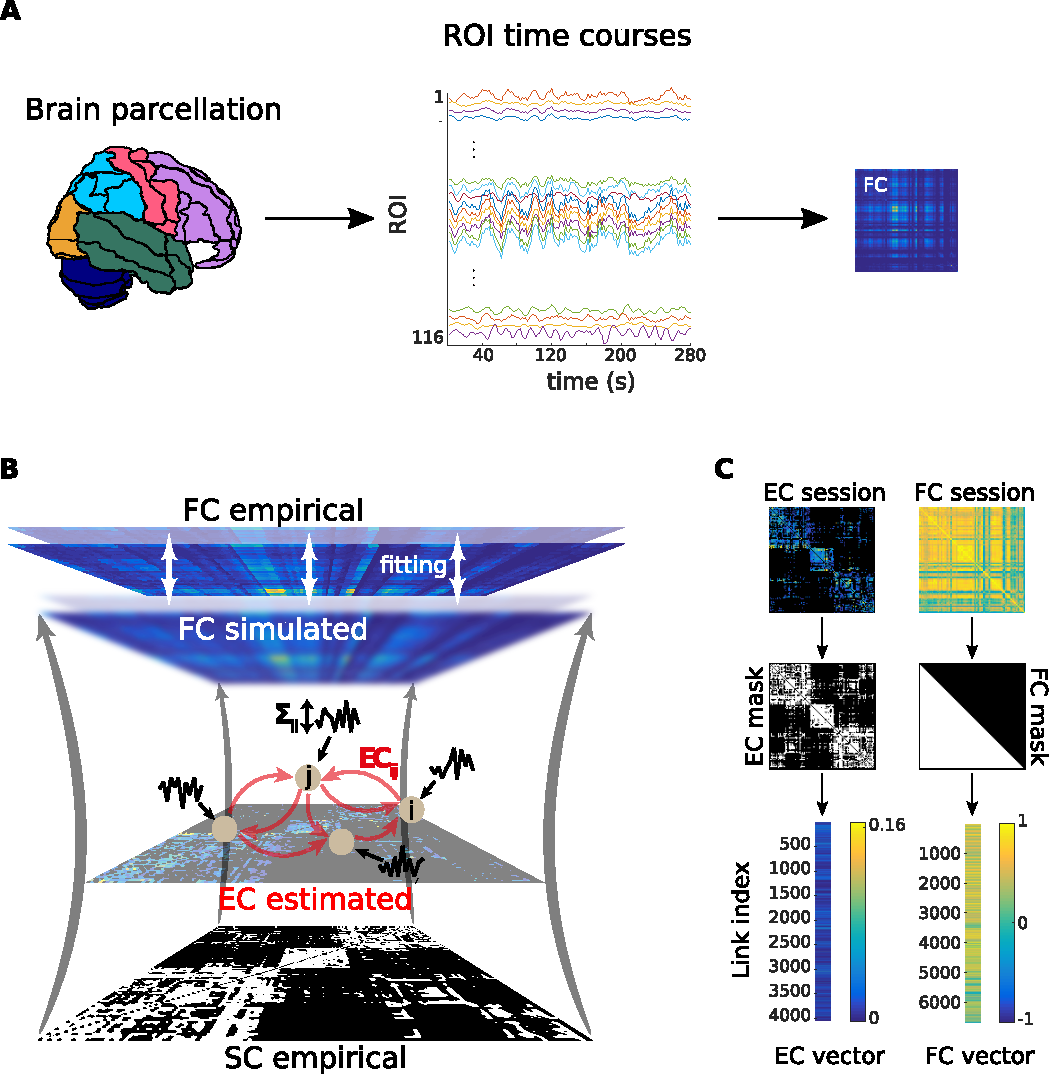
\includegraphics[width=0.9\columnwidth]{fig1}
	\caption{After a standard pre-processing pipeline, a parcellation
	covering the whole-brain is applied to extract BOLD time series with each
color representing an anatomical subsystem of several ROIs. 
B) Whole-brain network model. The local
fluctuating activity 
propagates via the recurrent EC to generate the correlation patterns at the
network level. The fitting procedure iteratively tunes EC and $\Sigma$
such that the model best reproduces the empirical FC. C) Each corrFC
matrix is symmetric and has all diagonal elements equal to 1, so that only 6670
independent links are retained for classification (lower
triangle). Likewise, the EC matrix has 4056 non-zero elements that are used in
the classification (density of 30\%).}
	\label{fig:fig1}
\end{figure}

\subsection{Subject identification}

Robust subject
identification for $\sim$100 subjects was pioneered by a recent publication [16],
relying on a k-nearest-neighbor (kNN) classifier with k=1 and PCC as metric.
In contrast with previous studies using 1NN [16,17,32], our method relies on a
multinomial logistic regression (MLR) classifier, a classical tool in machine
learning. MLR uses a linear model to predict the probability that an input
sample belongs to a class (subject here).

In classification algorithms the problem of overfitting describes the situation
where the algorithm performs very well with the data it is trained with, but
fails to generalize to new samples. Due to the high dimensionality of the
connectivity measures [29], it is essential to control for overfitting with an
appropriate training and test procedure. Our train-test procedure and the use
of large test-retest datasets – unlike previous studies [16,17,47] – aims to
provide a trustworthy characterization of the quality of the classifiers.
\glossarybox{z-score}{Transformation of a distribution that allows to highlight the fluctuations of
data around the mean.}
Figure \ref{fig:fig2}A describes the train-test procedure for the identification of
subjects: 1) fMRI sessions (EC in the figure) are randomly split in training
and test datasets; 2) after preprocessing (orange arrows) involving
within-session z-score followed – or not – by PCA,
the classifier is optimized as illustrated for the MLR with boundaries that
best predict the training dataset; 3) test set is used to verify the
generalization capability of the classifier (blue arrows), by measuring to
which extent the classifier boundaries, estimated with the train set, correctly
classify single sessions from the test set.
\glossarybox{PCA}{Technique that allows to reduce the dimensionality of a dataset by rotating and projecting the data in a new space.}

We first used Dataset A1 and increased the number of training sessions per
subject from 1 to 40 to evaluate how many training sessions are necessary for
satisfactory accuracy. As shown in Figure 3B, EC (in red) outperformed corrFC
(in blue) by more than one standard deviation (shaded area around the curve),
for both MLR and 1NN. Moreover, almost perfect classification was reached with
MLR for only 5 training sessions, whereas 10-15 were necessary for 1NN. This is
important when only a few training sessions per subject are available, as
expected with clinical applications. Figure 3C displays the classification
accuracy for Dataset B, used to verify the robustness with respect to the
number of subjects to be classified. We trained the classifiers with 1 session
per subject and evaluated the performance varying the number of subjects from 2
to 30 (test set comprised the remaining 9 sessions per subject). Again, EC is
more robust than corrFC: while performance with corrFC rapidly deteriorates as
the number of subjects is increased, classification using EC is barely affected
by the number of subjects. This is our core technical result: EC and MLR
largely outperform corrFC and 1NN, respectively.

\begin{figure}[htpb]
	\centering
	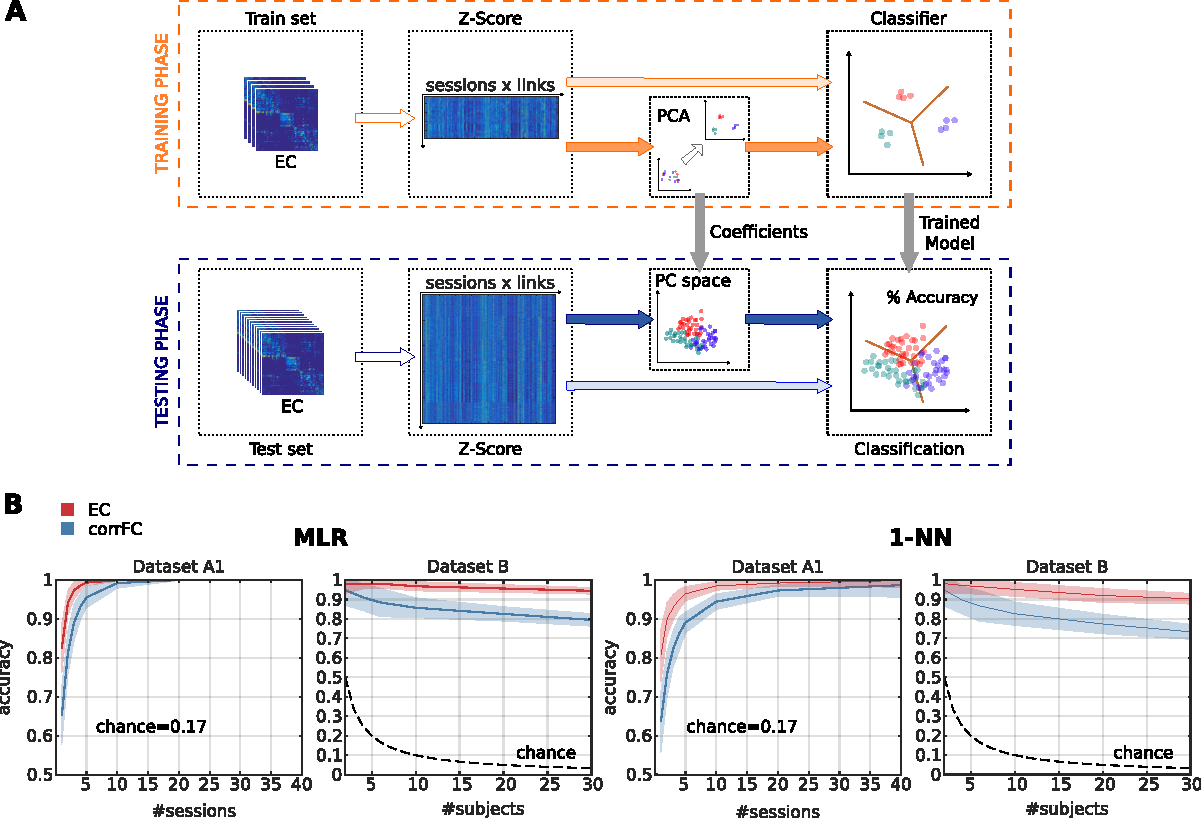
\includegraphics[width=0.9\columnwidth]{fig2}
	\caption{Subject identification using EC and FC. A) Classification
	pipeline used to assess the generalization of performance. The full set
of connectivity measures (here EC) over all fMRI sessions was split into two
groups: a train set and a test set. We use z-scores calculated over the
elements of each session matrix. We trained the
classifier – with or without previously applying PCA – and evaluated the
classification accuracy on the test set. B) Performance of multinomial logistic
regression (MLR, left panel) and 1-nearest-neighbor (1NN, right panel)
classifiers when increasing the number of sessions per subject used as training
set with Dataset A1. The mean (solid curve) and standard deviation (colored
area) were calculated for 100 repetitions with cross-validation. C) Same as B
when varying the number of subjects using Dataset B, using a single training
session per subject (leaving 9 sessions per subject as test test).}
	\label{fig:fig2}
\end{figure}


\subsection{Network of subject identification}
An important advantage of the MLR over kNN is its efficiency in
characterizing the links that contribute to the classification. We used
recursive feature elimination (RFE) to rank the links
according to their weight in the classification and then chose the lowest
number of links that achieved the maximum classification performance.
The resulting
support network for dataset A1 had 18 links, compared to 44 links for dataset
B. In both cases, subject identification using only those links achieved
perfect accuracy. The two support networks are shown in Figure
\ref{fig:fig3}A in the same matrix: remarkably, the networks are very sparse and
non-uniformly distributed across the whole brain. 
\glossarybox{Network}{A set of nodes connected by links. As shown below, network can be represented with dots and arrows or in matrix form, where each 
	element of the matrix correspond to one link and its value is 1 if the link exists or 0 if it doesn't.\\[0.5cm]
	
\includegraphics[width=0.9\columnwidth]{toy_net}}
This is the signature of the
most subject-discriminative ROIs: frontal and cingulate cortices, as well as
the temporal and occipital regions, seem to play a major role here. It is worth
noting that the adjacency matrix is not symmetric, which implies different
roles for nodes as receivers (especially frontal ROIs) or senders (cingulate).

\begin{figure}[htpb]
	\centering
	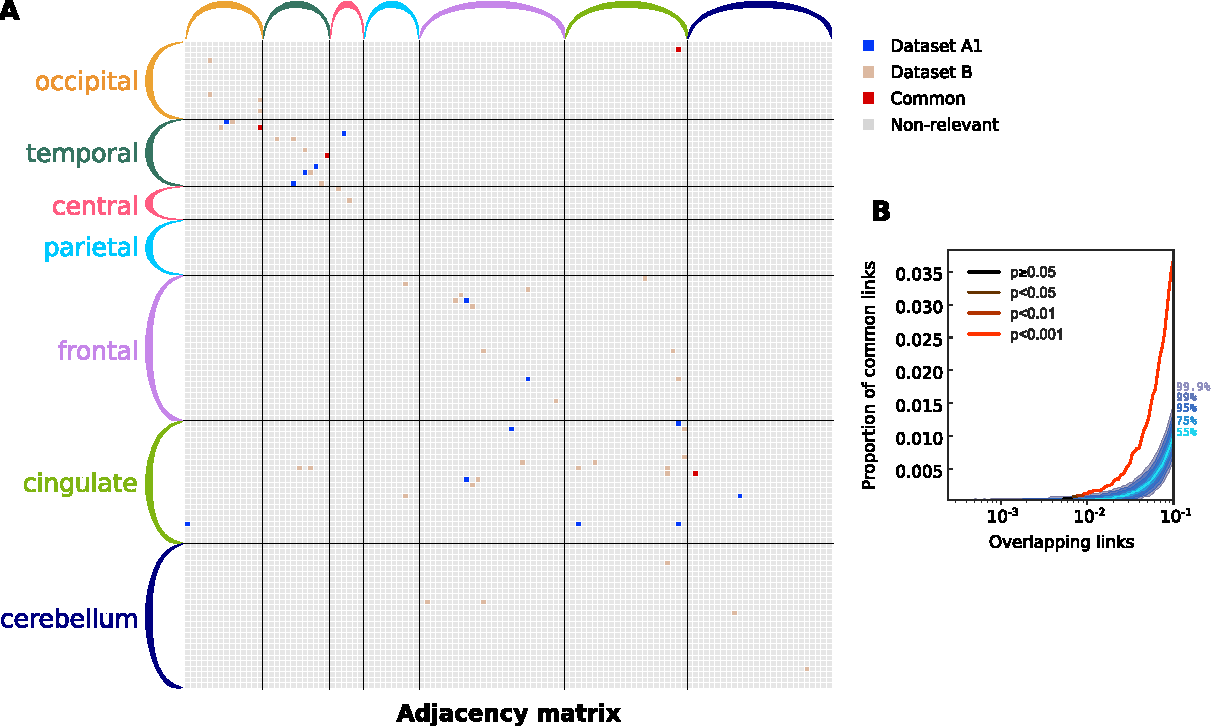
\includegraphics[width=0.9\columnwidth]{fig3}
	\caption{Networks that support subject identification. A) Extracted
links that contribute to the classification with both datasets, obtained using
recursive feature elimination (RFE). The ROIs are grouped in anatomical pools.
B) Overlap between the two signatures
for Datasets A1 and B as a function of selected links. The curve represents the
amount of common links in the data. Shaded areas represent different quantiles
of the surrogate distribution of common links under the null-hypothesis of
random rankings. The color of the curve indicates the probability of the
corresponding amount of common links under the null-hypothesis (here p-value <
0.001 when considering more than 1\% of the total links, namely 40 links).}
	\label{fig:fig3}
\end{figure}

The sparsity of the signature in Figure \ref{fig:fig3}A hides the fact that the rankings for
Datasets A1 and B are close (PCC=0.59, p-value<<10-50), indicating that similar
neural networks characterize individuals in two disjoint sets of subjects; see
also Figure \ref{fig:fig4} that illustrates the correspondence at the level of anatomical
groups. To further measure the overlap between these
networks, we selected the subset of links with the highest ranking for each
dataset and computed the number of common links. Figure 3E shows that the
proportion of common links exceeds by far its expectation under the hypothesis
of random rankings (shaded gray area). This indicates a good agreement between
the support networks from the two datasets even at the single-link level.

\begin{figure}[htpb]
	\centering
	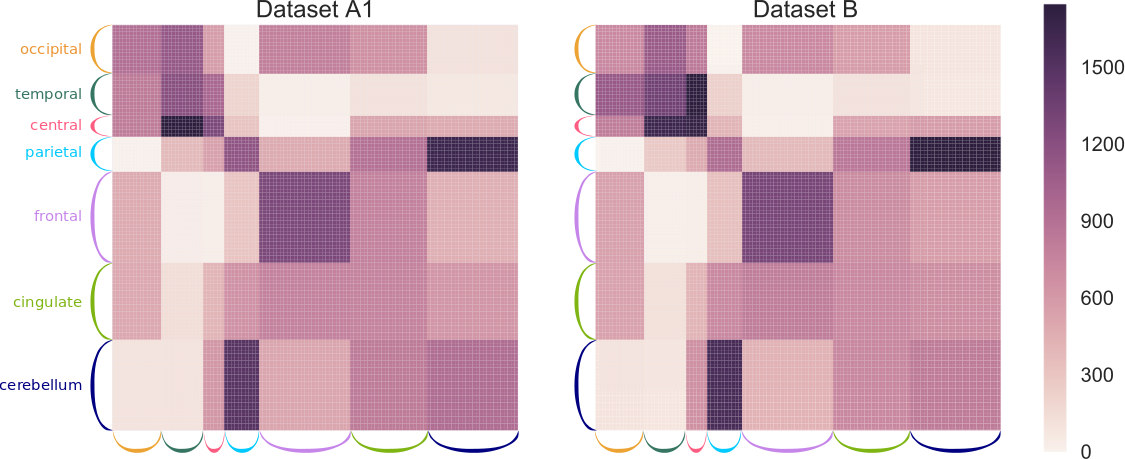
\includegraphics[width=0.9\columnwidth]{avg_ranking_subsystems.png}
	\caption{Correspondence of links at the level of subsystems. Number of links in each subsystem is represented by color for the two
	datasets A1 and B. The number of links for each subsystem is very similar between the two datasets.}
	\label{fig:fig4}
\end{figure}

\subsection{Condition identification and related network}

Finally, we used Dataset C to extract a signature for the subject identity and
another for the behavioral condition. This is schematically depicted in Figure
\ref{fig:fig5}A, with three fictive dimensions: the information about subject identity
corresponds to the x-axis and information about the condition to the z-axis;
the session-to-session variability, that should be ignored, spreads along the
y-axis. In this idealized low-dimensional scenario, it is possible to classify a session with
respect to both subjects and conditions using different planes of the data.
In the high dimensional case different hyperplanes would be used, in practice different sets of links support
the two classifications.  Using MLR and EC, we achieved very high performance
(accuracy $>$90\%) for subject identification and perfect classification for the
condition. 

We then sought the smallest subsets of links that achieved the maximum
performance of each classification using RFE (Figure \ref{fig:fig5}B), as done before.
Both support networks were again very sparse and
distributed across the brain, as can be seen in their adjacency matrix (Figure
\ref{fig:fig5}C). More links are necessary to identify the subjects (57) than the behavioral
conditions (13), indicating a higher complexity for the former.

Despite a (small) overlap of links between two networks, links relevant for subjects' identity and behavioral condition belong to almost disjoint
sets. In order to prove this point we used RFE to rank the links according to their contribution to the
classification, as we did before for datasets A1 and B. We computed the number of common links for the subject and
condition identifications, which fell within the expected values for the null
hypothesis (Figure \ref{fig:fig5}D). Thus the overlap at the level of individual links is not any larger than that 
expected by chance.

\begin{figure}[htpb]
	\centering
	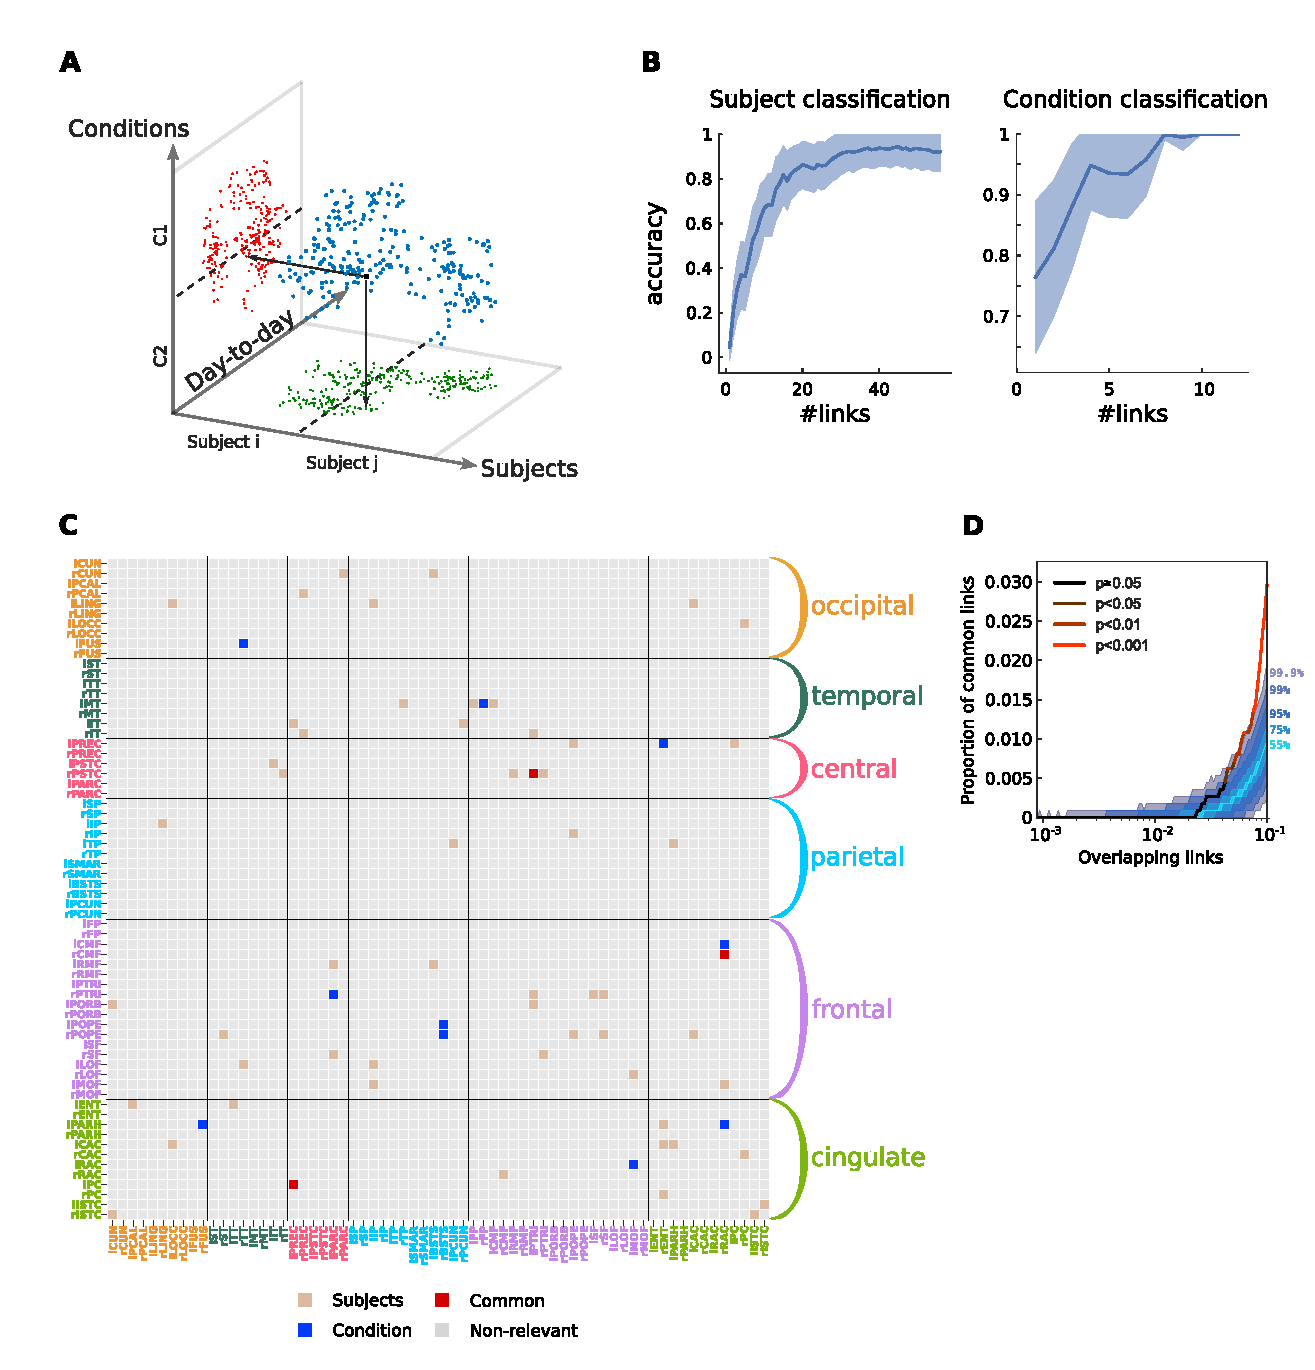
\includegraphics[width=0.9\columnwidth]{fig5}
	\caption{Twofold discrimination between subjects and conditions using EC.  A) Idealized
scheme of the twofold classification where each session (blue dots) is
“projected” onto two planes, one for subjects (green) and one for conditions
(red). In each plane, classification can be performed efficiently. Depending
on the orthogonality of the subspaces, the two signatures have more or less
overlap. B) Performance of the classification for 19 subjects and 2 conditions
using Dataset C as a function of number of links. C)
Signatures of the most discriminative EC links for the twofold classification: 54 links for subject
classification in brown, 10 for condition classification in blue, 3 common
links in red. D) Proportion of common links between the subject and
condition signatures as a function of selected links. Color coding is the same as in Figure \ref{fig:fig4}B.
}
	\label{fig:fig5}
\end{figure}

Similar to Datasets A1 and B, subject identification of Dataset C largely
concerns the frontal and cingulate systems. Condition identification is also
supported by occipital and temporal cortices, which are expected to have the
strongest activity modulations during movie viewing. The top panels in Figures
\ref{fig:fig6}A and B represent the two support networks such that the directed nature of
links can be appreciated. Apart from two small components, the subject network
appears almost fully connected with several central nodes (hubs, indicated by
their large size), located in frontal and cingulate regions. In comparison, the
condition network is segregated into small isolated components. The bottom
plots in Figure 5 show the lateralization of the support links, stressing the
asymmetries between the two hemispheres: most of the important links are
ipsilateral (i.e., within the same hemisphere) and many belong to the left
hemisphere for the subject network, whereas they are mainly contralateral for
the condition network.

\begin{figure}[htpb]
	\centering
	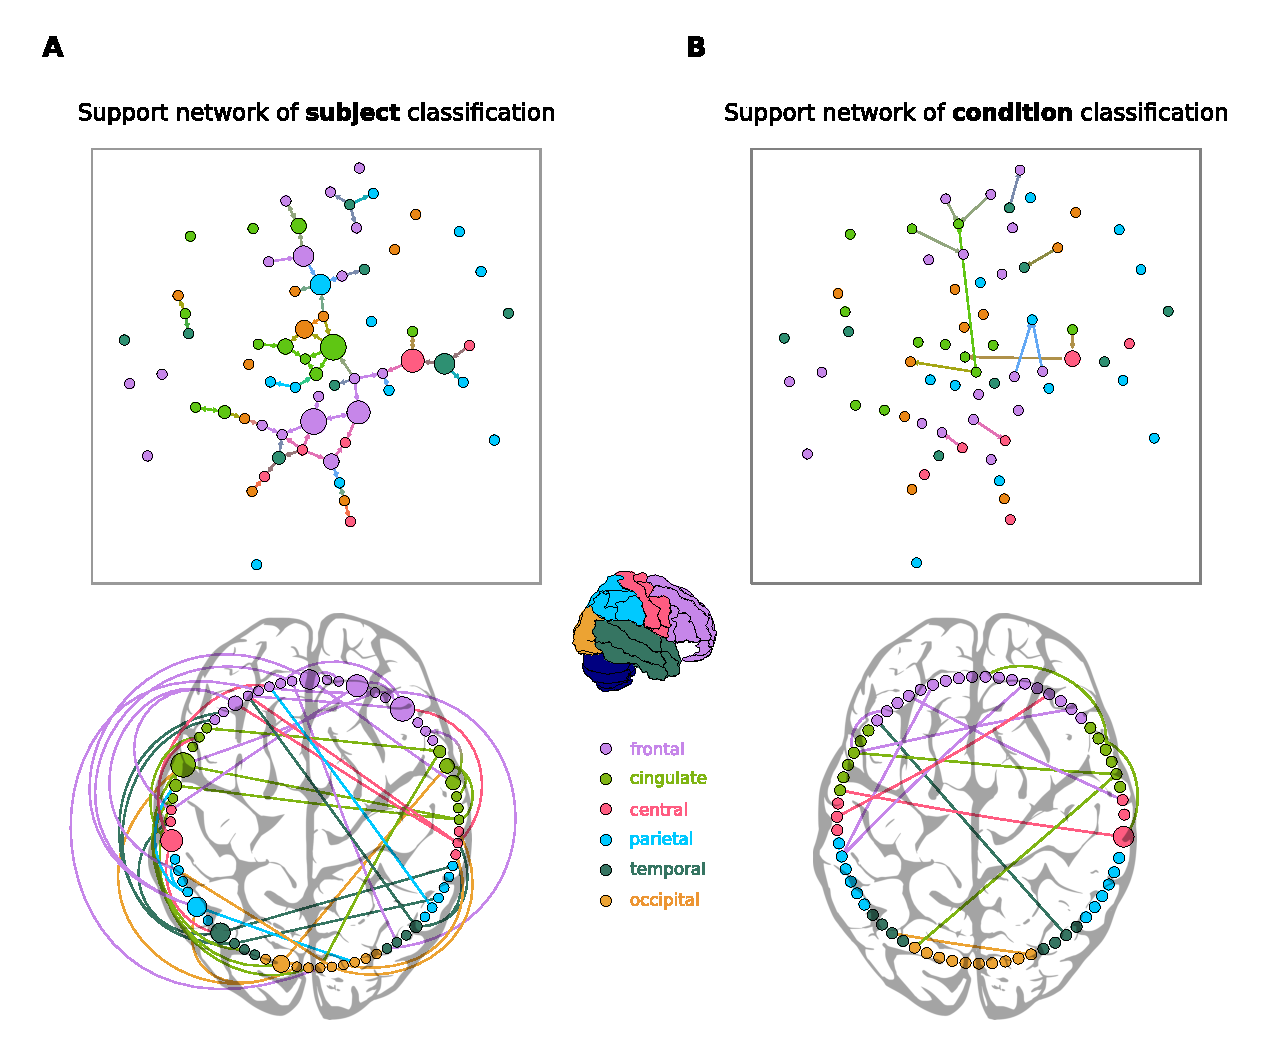
\includegraphics[width=0.9\columnwidth]{fig6}
	\caption{Support networks of subject and condition classification. A)
	The top graph plot represents the 57 most discriminative EC links
	supporting the classification of subjects (same as in Figure \ref{fig:fig5}C). The size of
each node represents its centrality in the extracted network (how much connected it is). The
most central regions are located mainly in the frontal and cingulate cortices.
The bottom circular plot shows the asymmetry and lateralization of the network,
with more links located in the left hemisphere. Links that are inside the
circle correspond to contralateral connections, while links outside the circle
correspond to ipsilateral connections. B) Similar graph and circular plots as A
for the 13 links supporting the classification between the two conditions.}
	\label{fig:fig6}
\end{figure}

\section{Next step: dynamic EC extraction}
\label{dynEC}

Summarizing here we presented a reliable method to classify simultaneously subjects and conditions and to extract 
the network underlying these classifications.
To the aim of applying this method to the study of different cognitive functions we foresee some necessary adaptations.
The typical timespan of cognitive tasks is usually less than one minute (even few seconds for very stereotyped perceptual
tasks). Our method is calibrated for fMRI sessions of few minutes. Even if experimental manipulations could provide experimental
tasks with longer time scales, an improvement of the method is necessary to allow the use of very short recording sessions.
The main limitation of the method is related to the estimation of EC. Indeed the estimation procedure relies on the calculation of
the correlation matrix. However when the number of ROIs is in the same order of the number of time points the correlation matrix will be
very noisy (not to mention the case when there are more ROIs than time points, for which the correlation matrix becomes singular).
Regularization is usually the solution to this type of problems, i.e. the pruning of the number of ROIs in this case.
Another approach, the one that we are currently following, is that of a Bayesian estimation of the EC. The Bayesian setting allows the use of
a prior probability on the EC that acts as a regularizer and allows a more robust estimation even when the number of time points is limited.

\end{document}
